\bta{电磁波}

\begin{enumerate}
	%\renewcommand{\labelenumi}{\arabic{enumi}.}
	% A(\Alph) a(\alph) I(\Roman) i(\roman) 1(\arabic)
	%设定全局标号series=example	%引用全局变量resume=example
	%[topsep=-0.3em,parsep=-0.3em,itemsep=-0.3em,partopsep=-0.3em]
	%可使用leftmargin调整列表环境左边的空白长度 [leftmargin=0em]
	\item
\exwhere{$ 2013 $ 年上海卷}
电磁波与机械波具有的共同性质是 \xzanswer{B} 

\fourchoices
{都是横波}
{都能传输能量}
{都能在真空中传播}
{都具有恒定的波速}


\item
\exwhere{$ 2014 $ 年物理上海卷}
下列电磁波中,波长最长的是 \xzanswer{A} 

\fourchoices
{无线电波}
{红外线}
{紫外线}
{$ \gamma $ 射线}



\item 
\exwhere{$ 2015 $ 年上海卷}
 $ X $ 射线 \xzanswer{B} 
 

\fourchoices
{不是电磁波}
{具有反射和折射的特性}
{只能在介质中传播}
{不能发生干涉和衍射}


\item 
\exwhere{$ 2014 $ 年理综四川卷}
电磁波已广泛运用于很多领域,下列关于电磁波的说法符实际的是 \xzanswer{C} 
\fourchoices
{电磁波不能产生衍射现象}
{常用的摇控器通过里出紫外先脉冲信号来摇控电视机}
{根据多普勒效应可以判断遥远天体相对于地球的运动速度}
{光在真空中运动的速度在不同惯性系中测得的数值可能不同}


\item 
\exwhere{$ 2013 $ 年四川卷}
下列关于电磁波的说法,正确的是 \xzanswer{C} 


\fourchoices
{电磁波只能在真空中传播}
{电场随时间变化时一定产生电磁波}
{做变速运动的电荷会在空间产生电磁波}
{麦克斯韦第一次用实验证实了电磁波的存在}



\item 
\exwhere{$ 2013 $ 年浙江卷}
关于生活中遇到的各种波,下列说法正确的是 \xzanswer{B} 

\fourchoices
{电磁波可以传递信息,声波不能传递信息}
{手机在通话时涉及的波既有电磁波又有声波}
{太阳光中的可见光和医院“$ B $超”中的超声波传递速度相同}
{遥控器发出的红外线波长和医院 $ CT $ 中的 $ X $ 射线波长相同}



\item 
\exwhere{$ 2015 $ 年理综北京卷}
利用所学物理知识,可以初步了解常用的公交一卡通($ I_{C} $ 卡)的工作原
理及相关问题。$ I_{C} $ 卡内部有一个由电感线圈 $ L $ 和电容 $ C $ 构成的 $ LC $ 振荡电路。公交车上的读卡机(刷
卡时“滴”的响一声的机器)向外发射某一特定频率的电磁波。刷卡时,$ I_{C} $ 卡内的线圈 $ L $ 中产生感应
电流,给电容 $ C $ 充电,达到一定的电压后,驱动卡内芯片进行数据处理和传输。下列说法正确的是 \xzanswer{B} 

\fourchoices
{$ IC $ 卡工作所需要的能量来源于卡内的电池}
{仅当读卡机发射该特定频率的电磁波时,$ IC $ 卡才能有效工作}
{若读卡机发射的电磁波偏离该特定频率,则线圈 $ L $ 中不会产生感应电流}
{$ IC $ 卡只能接收读卡机发射的电磁波,而不能向读卡机传输自身的数据信息}



\item 
\exwhere{$ 2016 $ 年北京卷}
下列说法正确的是 \xzanswer{A} 

\fourchoices
{电磁波在真空中以光速 $ c $ 传播}
{在空气中传播的声波是横波}
{声波只能在空气中传播}
{光需要介质才能传播}



\item 
\exwhere{$ 2016 $ 年上海卷}
各种不同频率范围的电磁波按频率由大到小的排列顺序是 \xzanswer{A} 

\fourchoices
{$ \gamma $射线、紫外线、可见光、红外线}
{$ \gamma $射线、红外线、紫外线、可见光}
{紫外线、可见光、红外线、$ \gamma $射线}
{红外线、可见光、紫外线、$ \gamma $射线}



\item 
\exwhere{$ 2016 $ 年天津卷}
我国成功研发的反隐身先进米波雷达堪称隐身飞机的克星,它标志着我国雷达
研究又创新的里程碑,米波雷达发射无线电波的波长在 $ 1 \sim 10 \ m $ 范围内,则对该无线电波的判断正确
的是 \xzanswer{C} 
% TODO: \usepackage{graphicx} required
\begin{figure}[h!]
	\centering
	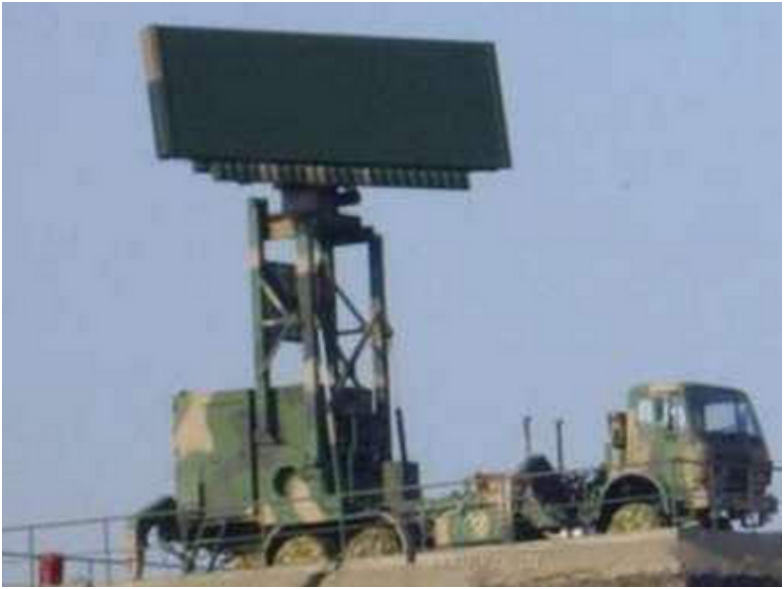
\includegraphics[width=0.17\linewidth]{picture/screenshot072}
\end{figure}

\fourchoices
{米波的频率比厘米波频率高}
{和机械波一样须靠介质传播}
{同光波一样会发生反射现象}
{不可能产生干涉和衍射现象}






	
	
	
\end{enumerate}

